\documentclass{article}
\usepackage{amsmath}
\usepackage{graphicx}
\begin{document}
\title{Quiz: Question 6}
\author{Ana Bhattacharjee}
\date{\today}
\maketitle

\begin{center}
To find the measure of angle A, we have to use the law of cosines. See the following visualization.
\begin{figure}[!htbp]
  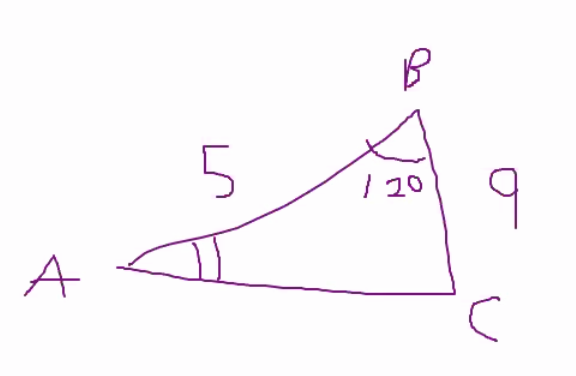
\includegraphics[width=1.0\columnwidth]{triangle}
  \caption{Triangle ABC}
\end{figure}
\begin{align}
b^2 = 5^2 + 9^2 - 2(5*9*cos(120)) \\
b^2 = 106 - 90cos(120) \\
b = \sqrt{106 - 90cos(120)} \approx 12.3 \\
9^2 = 5^2 + (12.3)^2 - 2(5)(12.3)cos(A) \\
81 = 25 + 151.3 - 123cos(A) \rightarrow 176.3 - 123cos(A) \\
cos(A) = -\frac{81 - 176.3}{123} \\
A = cos^{-1}(-\frac{81 - 176.3}{123}) \approx 141^{\circ}
\end{align}
Since the angle is across the side which is not the largest, we must subtract this answer from $180^{\circ}$ .
\begin{align}
  A = 180 - 141 \\
  A = 39^{\circ} 
\end{align}
\end{center}
\end{document}
